\section{Related Work}
\subsection{Generative Adversarial Networks}
    There exist a great deal of generative neural networks, for example Deep Boltzmann Machines, Variational Autoencoders and Generative Adversarial Networks, to name just a few. Nevertheless, the latter has to have something to it, since it has gotten a lot of hype recently and was even described by Yan LeCun as "the coolest idea in machine learning in the last 20 years"\footnote{https://www.youtube.com/watch?v=IbjF5VjniVE}. GANs have many use cases, including encryption, data manipulation and testing of security systems. However, the most popular use case is the generation of images.
    
\subsection{How does a GAN work}
	%how does a GAN work
	For this task of image generation, we make use of Generative Adversarial Networks. A GAN belongs to the class of the generative neural networks. GANs consist of two deep neural networks, commonly called Generator and Discriminator with respect to their adversarial task. They are trained by playing a min-max zero sum game where each loss is depending on the actions of the other network. The Generator maps a probability distribution to a visual output in form of multi-dimensional tensor. The Discriminator on the other hand provides feedback on the multi-dimensional output of the Generator by mapping it back to a probability distribution. \\
	
	\begin{figure}[htb] 
    	\centering
    	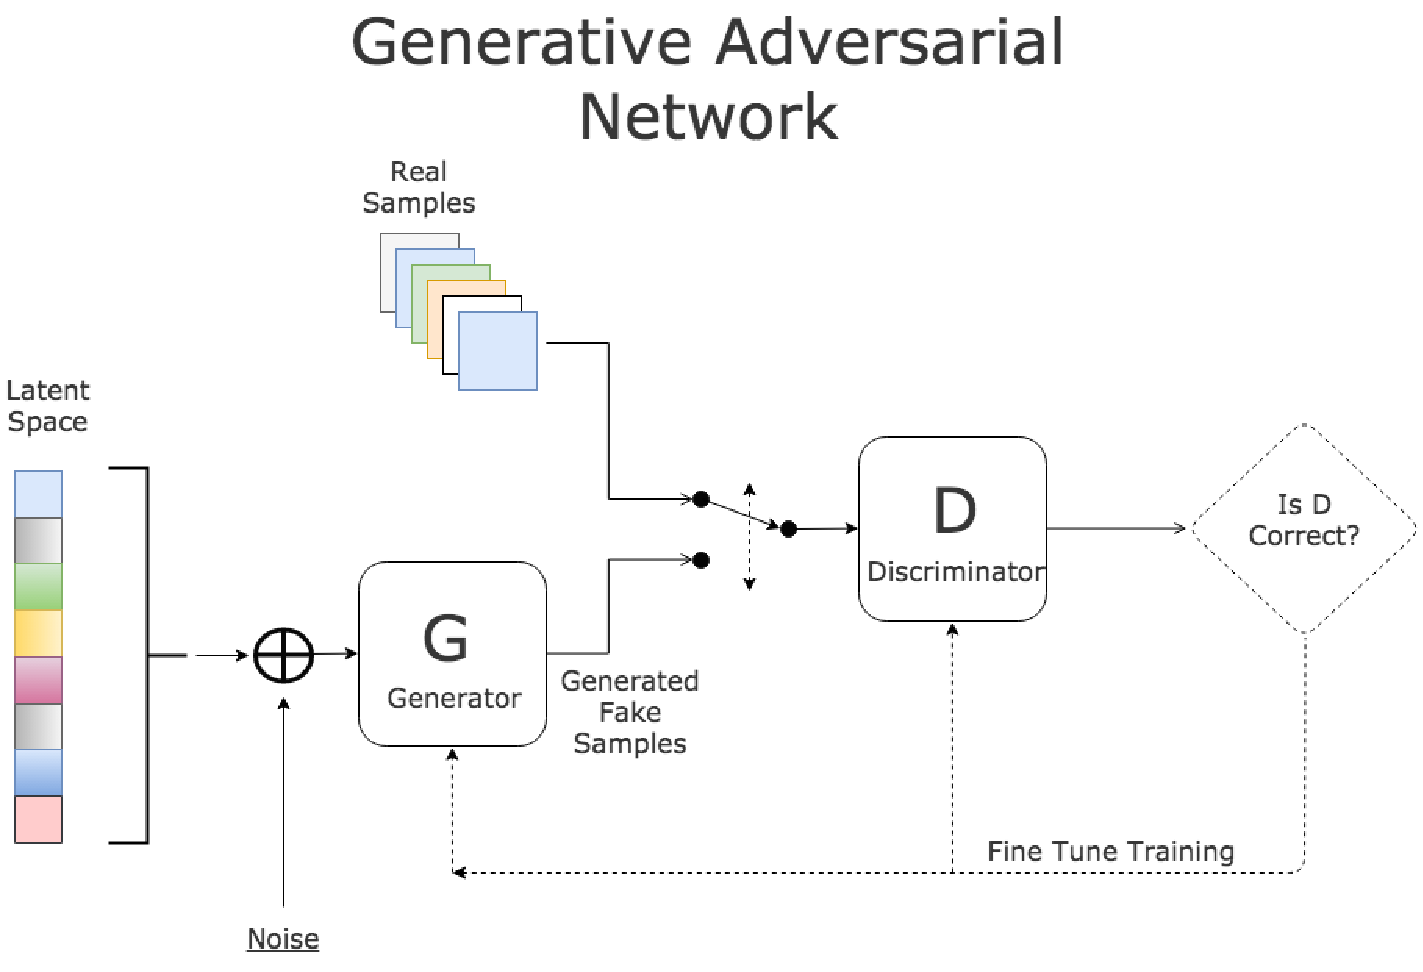
\includegraphics[width=0.7\linewidth]{GAN_structure.pdf}
    	\caption{Discriminator and Generator in the context of GANs}
    	\label{fig:GAN}
    \end{figure}
	\footnote{https://medium.com/ai-society/gans-from-scratch-1-a-deep-introduction-with-code-in-pytorch-and-tensorflow-cb03cdcdba0f}
	
	Hereby, the Discriminator assigns probabilities to each class the generated image might belong to. As we consider a binary decision between 0 and 1, the final layer of the Discriminator will be a single neuron. The Generator does not have direct access to the real data that it should eventually be able to create instances of, but the Discriminator does as he is fed with fabricated input from the Generator and real samples. Hence, the Discriminator tells the Generator about the quality of the learnt features indirectly through its loss function. By iteratively incorporating the provided feedback the Generator will ultimately produce outputs that the Discriminator cannot distinguish from the real samples which leads to the Discriminator outputting a probability of 0.5 for any generated image created by the Generator.  
    %who started this idea
    GANs were first introduced by Ian Goodfellow \cite{goodfellow2014generative} in 2014. The Generator G tries to minimize the value while the Discriminator D tries to maximize it. The formula depicting this behaviour looks as follows: 

    \begin{equation}
        \min_{D} \min_{G} V(D,G) = \mathbb{E}_{x \sim p_\textbf{data}(x)}[\log D(x)] + \mathbb{E}_{z \sim p_\textbf{z}(z)}[1-\log D(G(z))]
    \end{equation}
    
\subsection{Unpaired Image-to-Image Translation}
    At the end of 2018, Jun-Yan Zhu et al. published an authoritative paper dealing with unpaired image to image translation \cite{zhu2017unpaired}.
    In this paper, image to image translation is defined as follows: image-to-image translation is a class of vision and graphics problems where the goal is to learn the mapping between an input image and an output image using a training set of aligned image pairs.\\
    This implies having paired image data, since images of the same object are required by the source and the target domains. This confronts us with the problem of data availability. In many areas, collecting images in pairs is either extremely difficult (images of houses before flooding) or even impossible (in the case of deceased artists who obviously will not draw new paintings that you could use).\\
    Therefore, Jun-Yan Zhu et al. introduce an extension of the Generative Adversarial Network, namely the Cycle-Consistent GAN. With the help of a consistency loss an attempt is made to increase the quality of the images. Given are two projections G: X$\,\to\,$Y and F: Y$\,\to\,$X, where X and Y represent domains. For an input x the loss is calculated from the difference between x and F (G (x)) and thus minimizing the loss will result in more accurate and vivid representation of the observable world.\\
    The use of two mappings instead of one and the introduction of the cycle consistency loss is the main difference to a standard GAN. Since we map bidirectionally between domains, we need two additional loss functions, one for the forward cycle consistency and one for the backward cycle consistency:
    
    \begin{multline}
                \L_{cyc}(G,F) =  
        \mathbb{E}_{x \sim p_\textbf{data}(x)}
        [ \lVert F(G(x)) - x \rVert_{1} ] + \\
        \mathbb{E}_{y \sim p_\textbf{data}(y)}
        [ \lVert F(G(y)) - y \rVert_{1} ]
    \end{multline}
    
        
    \subsection{Visualizing Climate Change}
        If you research CCGAN, you will primarily get to see beautifully fabricated images of winter landscapes or fails that happen when horses are transformed into zebras. Viktor Schmidt et al. \cite{schmidt2019visualizing} present another interesting approach in this year's paper, which is intended to illustrate the dimensions of climate change to people.\\
        Using climate predictions, they tried to realistically represent the effects that would occur within 50 years. They initially limited themselves to a flooding scenario, i.e. simulating houses in the event of inundation. However, their declared goal is to extend the forecast to other domains later on. Nevertheless, this scenario alone is already relatively intricate. Since there is no database with pictures for such a case, they were searched manually on the web. In addition, only images with almost no external factors have proven useful. Their dataset consists of detached houses with a garden or greenspace in the foreground. \\
        Their work eventually got our interest and made us initiate the project we will describe in the following sections.